%
% Slide template for LSIII presentations
%

%\documentclass[10pt,landscape,handout]{beamer}
%\documentclass[10pt,landscape,draft]{beamer}
\documentclass[10pt,landscape]{beamer}


% Be able to directly input German Umlauts etc.
%\usepackage[latin1]{inputenc}

% Font encoding:
\usepackage[T1]{fontenc}
\usepackage{lmodern}
\usepackage[utf8]{inputenc}
\usepackage{german}
\usepackage{ragged2e}
\usepackage{epstopdf}
\usepackage{amssymb}
\usepackage{amsmath}
\usepackage{stackengine}
% We recommend toying around with these settings,
% No overridden font encoding looks best,
% unless you are using \textsc (which will default to CMF).


% the usual imports
\usepackage{graphicx}


% setup beamer style to use TUDo Theme
\mode<presentation>
{
  \usetheme{TUDortmund}
}

% Include intermediate TOCs automatically.
% Completely pointless for these slides, however
%\AtBeginSection[]
%{
%  \begin{frame}<beamer>
%    \frametitle{\"Ubersicht}
%    \tableofcontents[currentsection]
%  \end{frame}
%}

%
% Options for navigation symbols
%
% a) Small set of navigation symbols
%\setbeamertemplate{navigation symbols}{
%  \insertbackfindforwardnavigationsymbol
%  \hspace{0.5em}
%  \insertslidenavigationsymbol
%  \insertframenavigationsymbol
%  \insertsubsectionnavigationsymbol
%  \insertsectionnavigationsymbol
%  \insertdocnavigationsymbol
%  \hspace*{\textwidth}\hspace*{0.2cm}
%}
%
% b) Suppress navigation symbols
\setbeamertemplate{navigation symbols}{}

\newcommand{\lc}[1]{\texttt{\textbackslash#1}}
\newcommand{\lcp}[2]{\texttt{\textbackslash#1\{#2\}}}
\newcommand{\lco}[2]{\texttt{\textbackslash#1[#2]}}
\newcommand{\lcop}[3]{\texttt{\textbackslash#1[#2]\{#3\}}}
\newcommand{\lcpp}[3]{\texttt{\textbackslash#1\{{#2}\}\{{#3}\}}}
\newcommand{\lcppp}[4]{\texttt{\textbackslash#1\{#2\}\{#3\}\{#4\}}}
\newcommand{\lcopp}[4]{\texttt{\textbackslash#1[#2]\{#3\}\{#4\}}}
\newcommand{\lenv}[2]{\texttt{\textbackslash{}begin\{#1\}\linebreak[0]#2\linebreak[0]\textbackslash{}end\{#1\}}}

\newcommand{\todo}[2]{\colorbox{orange}{\textbf{#1:} {#2}}}
\newcommand{\ds}{\ensuremath\displaystyle}
\newenvironment{determinante}[1]{%
\ensuremath\left|\begin{array}{#1}}{%
\end{array}\right|}

%%%%%%%%%%%%%%%%%%%%%%%%%%%%%%%%%%%%%%%%%%%%%%%%%%%%%%%%%%%%%%%%%%%%%
%%% Basic information
%%%%%%%%%%%%%%%%%%%%%%%%%%%%%%%%%%%%%%%%%%%%%%%%%%%%%%%%%%%%%%%%%%%%%


\title{AR Billiard mit OpenCV und OpenGL}
 

\subtitle{Sommersemester 2018}

\author{Friedemann Runte, Moritz Ludolph, Diyar Omar, Robin Mertens} 

\institute[Fakultät für Informatik, TU Dortmund]{Fakultät für Informatik}
\date{\today}


\begin{document}
\logo{}
\setlength{\parskip}{1mm}

%%%%%%%%%%%%%%%%%%%%%%%%%%%%%%%%%%%%%%%%%%%%%%%%%%%%%%%%%%%%%%%%%%%%%
%%% Title
%%%%%%%%%%%%%%%%%%%%%%%%%%%%%%%%%%%%%%%%%%%%%%%%%%%%%%%%%%%%%%%%%%%%%


% slide options are: alignment: c(enter) or t(op), label
\begin{frame}[c,label=titlepage]
  \titlepage
\end{frame}


%%%%%%%%%%%%%%%%%%%%%%%%%%%%%%%%%%%%%%%%%%%%%%%%%%%%%%%%%%%%%%%%%%%%%
%%% Overview
%%%%%%%%%%%%%%%%%%%%%%%%%%%%%%%%%%%%%%%%%%%%%%%%%%%%%%%%%%%%%%%%%%%%%


%\begin{frame}[t, label=overview]
  %\frametitle{\"Ubersicht}
  %\setcounter{tocdepth}{2}
  %\tableofcontents
%\end{frame}


%%%%%%%%%%%%%%%%%%%%%%%%%%%%%%%%%%%%%%%%%%%%%%%%%%%%%%%%%%%%%%%%%%%%%
%%% Global structure is declared through the usual section and 
%%% subsection environments. Starred sections will not appear in the 
%%% auto-generated TOCs.
%%%%%%%%%%%%%%%%%%%%%%%%%%%%%%%%%%%%%%%%%%%%%%%%%%%%%%%%%%%%%%%%%%%%%

\begin{frame}{Rendering und Phsyik}
\end{frame}
\begin{frame}{Darstellung des Spielfeldes}
\begin{itemize}
	\item Hintergrundfarbe Dunkel-Grün mit der OpenGL ClearColor
	\item Löcher und Kugeln mit Triangle-Fan
\end{itemize}
\end{frame}
\begin{frame}{Triangle-Fan}
\begin{itemize}
	\item Struktur aus Dreiecken
	\item Mittelpunkt $c$
	\item Radius $r$
	\item Auflösung $k$ ist die Anzahl der Dreiecke, aus denen unser Kreis hinterher besteht
\end{itemize}
\end{frame}
\begin{frame}
\begin{figure}
	\caption{Erstes Dreieck eines Triangle-Fans, i = 1, k = 36}
	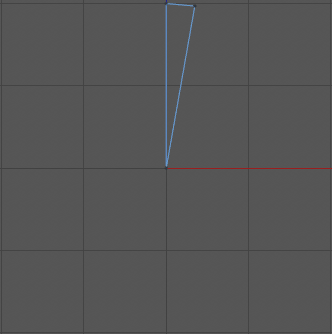
\includegraphics[width =150pt]{bilder/1.png}
\end{figure}
\end{frame}
\begin{frame}
\begin{figure}
	\caption{i = 2, k = 36}
	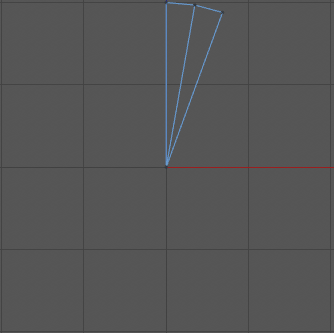
\includegraphics[width =150pt]{bilder/2.png}
\end{figure}
\end{frame}
\begin{frame}
\begin{figure}
	\caption{i = 3, k = 36}
	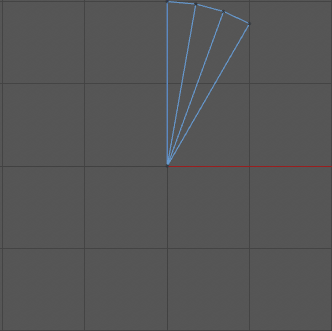
\includegraphics[width =150pt]{bilder/3.png}
\end{figure}
\end{frame}
\begin{frame}
\begin{figure}
	\caption{Vollständiger Triangle-Fan, i = k = 36}
	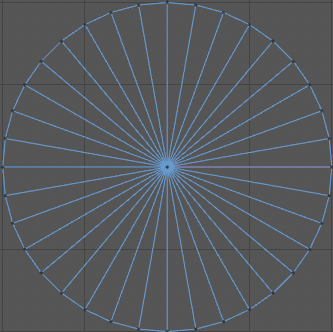
\includegraphics[width =150pt]{bilder/full.png}
\end{figure}
\end{frame}
\begin{frame}{Zwischenstand}
Wir haben nun ein Spielfeld mit Löchern und Kugeln. Jedoch sind die Kugeln noch nicht voneinander zu unterscheiden.
\begin{figure}
	\caption{Spielfeld ohne Texturen}
	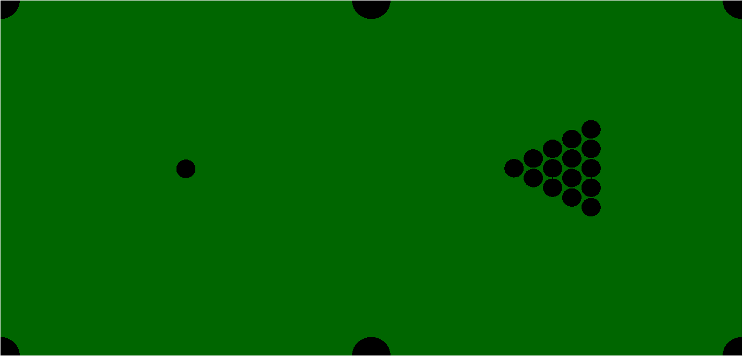
\includegraphics[width=250pt]{bilder/untextured_pool_low.png}
\end{figure}
\end{frame}
\begin{frame}{Texturierung}
Grundkonzepte:
\begin{itemize}
	\item Eine Textur besteht aus Koordinaten auf der u (waagerecht) und der v (vertikal) Achse
	\item Die beiden Achsen sind immer im Bereich $[0,1]$, egal wie groß die Textur ist
	\item Man gibt beim Erstellen von Objekten für jeden Knoten die Texturkoordinaten in u und v an, um sie auf das Objekt abzubilden
\end{itemize}
\end{frame}
\begin{frame}{Texturierung}
\begin{figure}
	\caption{Textur mit u- und v-Achse}
	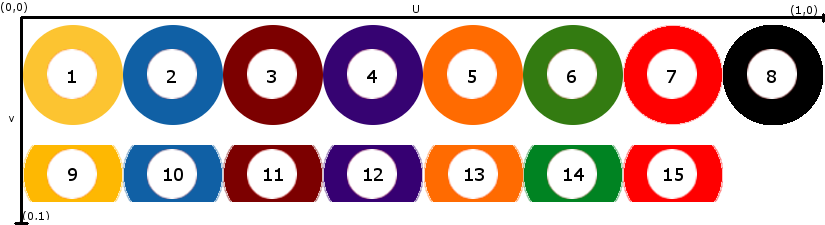
\includegraphics[width=250pt]{bilder/ballsachsen.png}
\end{figure}
Es fällt auf, dass eine Kugel $\frac{1}{8}$ Durchmesser hat auf u, aber $\frac{1}{2}$ auf v
\end{frame}
\begin{frame}{Texturierung}
Wir müssen nun berechnen, welcher Ausschnitt für welche Kugel ist.
	\begin{itemize}
		\item Die Farben sind geordnet auf der Textur und bekommen Werte von 0 bis 7
		\item Die Vollen Kugeln sind in der ersten Reihe und die Halben in der Zweiten und bekommen damit die Werte 0 (voll) und 1 (halb)
		\item Wir können jetzt eine Funktion erstellen, die uns anhand von Farbe und Fülle den Textur Mittelpunkt ausgibt 
	\end{itemize}
\end{frame}

\begin{frame}{Zwischenstand}
Wir haben nun ein fertiges Spielfeld mit Texturierten Kugeln.
\begin{figure}
	\caption{Fertiges Spielfeld}
	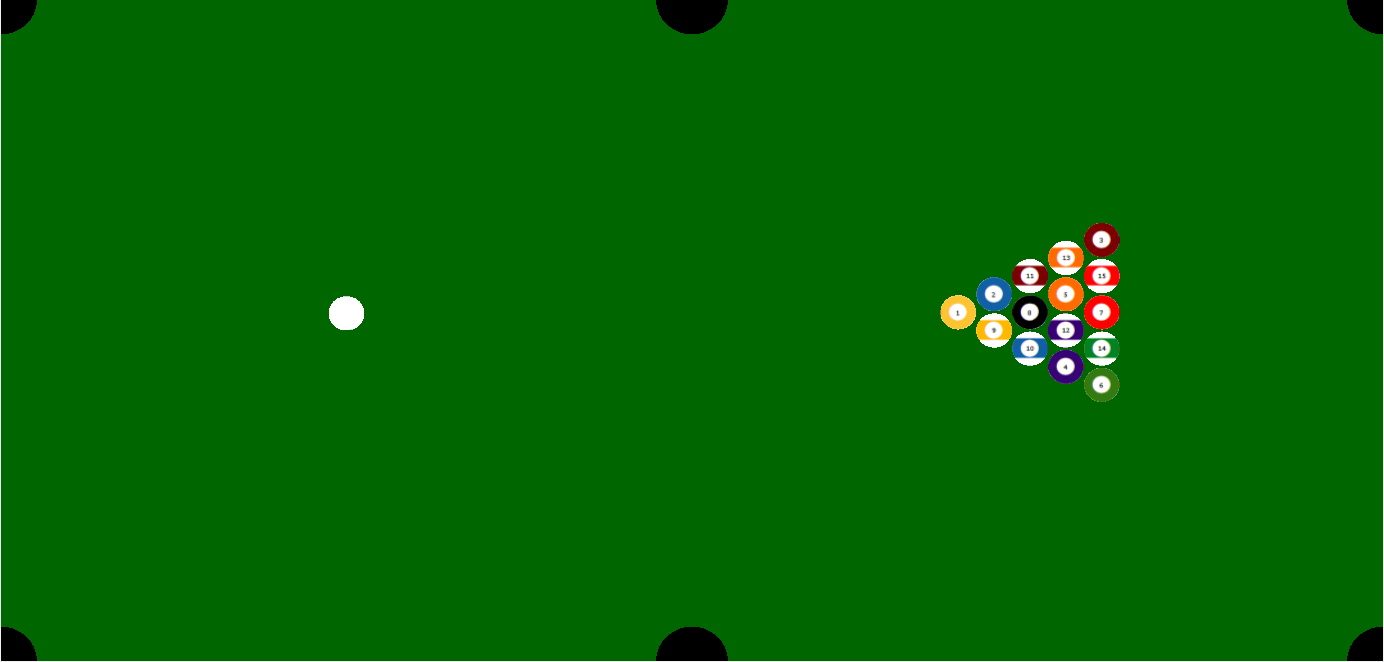
\includegraphics[width=300pt]{bilder/Spielfeld.png}
\end{figure}
\end{frame}
\begin{frame}{Physik}
Die Physik-Berechnungen des Spiels lassen sich aufteilen in 3 Bereiche:
\begin{itemize}
	\item Kollision von Kugel und Wand
	\item Kollision von Kugeln mit anderen Kugeln
	\item Kollision vom Queue mit der weißen Kugel
\end{itemize}
\end{frame}
\begin{frame}{Kollisionen: Kugel mit Wand}
Prinzip sehr einfach:
\begin{itemize}
	\item [1.] Definiere die Wände als Achsenabschnitte: Linke Wand ist $x=0$, rechte Wand $x=w$, obere Wand $y=0$ und untere Wand $y=h$, mit $w = $ Breite des Spielfeldes und $h = $ Höhe des Spielfeldes
	\item [2.] Überprüfen ob eine der Koordinaten der Kugel zusammen mit dem Radius eine der Wände schneidet \\
				z.B. für $r=5$ wäre $x = 5 - r = 0 $ und würde somit die Linke Wand schneiden
	\item [3.] Geschwindigkeit auf der Achse die Geschnitten wurde invertieren, also bei $x=0$ oder $x=w$ wird $vx = -vx$ gesetzt, analog für y
\end{itemize}
\end{frame}


\begin{frame}{Kollision mit anderen Kugeln}
\begin{itemize}
	\item Die Kollision von 2 Kreisen war uns bereits gegeben durch das Airhockey-Spiel.
	\item In Airhockey kollidiert ein Puck mit einem der beiden Schläger und bekommt dadurch eine neue Geschwindigkeit
	\item Der Schläger wird von der Kollision nicht verändert
	\item Wir brauchen aber, dass sich beide Kugeln bei Kollision verändern
\end{itemize}
\end{frame}
\begin{frame}{Kollision mit anderen Kugeln}
Lösung:
\begin{itemize}
	\item Wir berechnen für jede Kugel die Kollision mit jeder anderen Kugel
	\item Wir nehmen die Methode aus dem Airhockey und wählen unsere Kugel die sich bewegen soll als Puck und berechnen die Kollision mit allen anderen Kugeln als Schläger
	\item Wenn wir das in beide Richtungen ausführen, sodass jede Kugel sozusagen einmal Schläger und einmal Puck ist, wird jede Kugel von einer Kollision getroffen 
\end{itemize}
\end{frame}
\begin{frame}{Kollision mit Queue}
Die eigentliche Kollision bleibt gleich wie beim Airhockey. \\
\textbf{Problem: Framerate der Kamera} \\
$\implies$ Unschärfe lässt Kollisionen verloren gehen \\
Wird Später im Kontext des Queues erläutert.
\end{frame}
\begin{frame}{Kamerakalibrierung}
\end{frame}

\begin{frame}{Darstellung des Erkennungsmusters}
	Um die Kamera kalibrieren und das Kamerabild bzw. die -punkte entzerren zu können, muss die Kamera ein bekanntes Erkennungsmuster finden und in diesem bestimmte Eckpunkte erfassen und auswerten können.
	\pause
	\begin{itemize}
		\item[1.] Anzahl der Kacheln in der $Vertikalen$ und $Horizontalen$
		\item[2.] Höhe und Breite der Kacheln\\
		\pause
		$\implies$ $Hoehe_{Kachel} = \frac{Hoehe_{Game}}{Vertikalen}$, $Breite_{Kachel} = \frac{Breite_{Game}}{Horizontalen}$\\
		\pause
		\item[3.] Kacheln Rendern:\\
				$\implies$ Oben Links: ($i \cdot Hoehe_{Kachel}$, $j \cdot Breite_{Kachel}$)\\
				$\implies$ Unten Rechts: ($(i+1) \cdot Hoehe_{Kachel}$, $(j+1) \cdot Breite_{Kachel}$)\\
		\pause
		\item[4.] Damit das klassische Schwarz-Weiß-Muster eines Schachbretts visualisiert wird muss man:\\
		$\implies$ Kacheln in der Horizontalen die invertierte Farbe der vorherigen Kachel als Grundfarbe wählen und \\
		$\implies$ Kacheln in der Vertikalen für die erste Kachel die invertiere Farbe der darüber liegenden Kachel wählen
	\end{itemize}
\end{frame}
\begin{frame}{Darstellung des Erkennungsmusters}
	\begin{figure}[h]
		\centering
		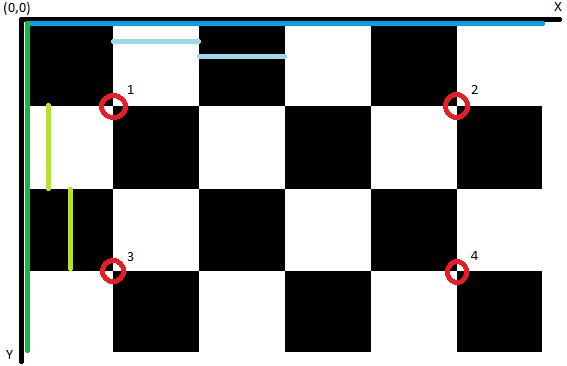
\includegraphics[scale=0.5]{bilder/schachbrett.png}
	\end{figure}

\end{frame}

%###########################

\begin{frame}{Entzerrung des Kamerabildes/Punktes}
Für die Kalibrierung des Kamerabildes mittels eines Patternmusters, muss zwischen zwei Ansichten unterschieden werde
	\begin{itemize}
		\item Weltkoordinaten = Patternkoords. ideal/entzerrt
		\item Bildkoordinaten = Patternkoords. aus aufgenommenem Bild/verzerrt
	\end{itemize}
\end{frame}

\begin{frame}{Weltkoordinaten erstellen}
	Da die übergebenen Punkte nachher in ein 2D-Koordinatensystem, das vom Spiel, dargestellt werden sollen, werden die Erkennungspunkte des Schachbrettmusters als 2D-Punkte gespeichert:\\
	$WeltCoords = (x \cdot a, y \cdot a, 0)$\\
	$a$ = Kantenlänge, $x \in [0,Vert-1], y \in [0,Hort-1]$\\
\end{frame}

\begin{frame}{Kalibrierungsparameter berechnen}
	\[s
	\begin{bmatrix}
	u\\v\\1
	\end{bmatrix}=
	\begin{bmatrix}
	f_{x} & 0 & c_{x}\\
	0 & f_{y} & c_{y}\\
	0 & 0 & 1
	\end{bmatrix}
	\begin{bmatrix}
	r_{11} & r_{12} & r_{13} & t_{1} \\
	r_{21} & r_{22} & r_{23} & t_{2} \\
	r_{31} & r_{32} & r_{33} & t_{3}
	\end{bmatrix}
	\begin{bmatrix}
	X\\Y\\Z\\1
	\end{bmatrix}
	\]
\end{frame}

\begin{frame}{Kalibrierungsparameter berechnen}
	Eingabe:\\
	\begin{itemize}
		\item Bildkoordinaten 2D Matrix\\
		\item Weltkoordinaten 3D Matrix\\
		\item Anzahl vertikaler und horizontaler Fixpunkte im Schachbrett
	\end{itemize}
\end{frame}

\begin{frame}{Kalibrierungsparameter berechnen
	\begin{figure}[h]
		\centering
		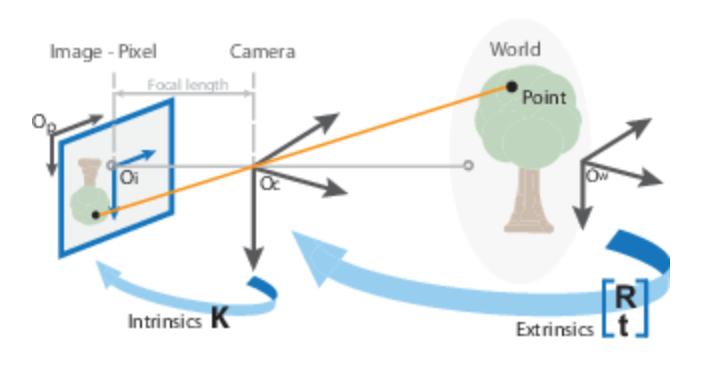
\includegraphics[scale=1.3]{bilder/extrinIntrin.PNG}
	\end{figure}
	Nun erhalten wir die extrinsischen ("äußeren"), sowie die intrinsischen ("inneren") Entzerrungsparameter
\end{frame}

%###########################

\begin{frame}{Punktübertragung von Kamera ins Spiel}
	Der letzte Abschnitt der Kamerakalibrierung stellt das Übertragen eines von der Queue-Erkennung gegebenen Punktes ins Spielfeld da. Um dies einwandfrei zu ermöglichen, müssen folgende Punkte erfüllt werden:
	\begin{itemize}
		\item[1.] äußersten Eckpunkte des, von der Kamera erfassten bilder bekannt sein\\
		$\implies$ die ganz äußersten Eckpunkte wie folgt berechnet werden:
		$\implies$ $Lila_{min} = Gruen_{min} - Rot_{min}$, $Lila_{max} = Rot_{max} - Gruen_{max}$
		\pause
	\end{itemize}	
\end{frame}

\begin{frame}{Punktübertragung von Kamera ins Spiel}
		\begin{figure}[h]
		\centering
		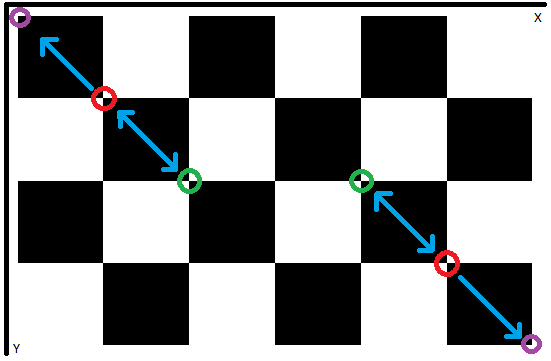
\includegraphics[scale=0.5]{bilder/schachbrettdiff.png}
		\caption{Schachbrettmuster Eckpunkte}
	\end{figure}
\end{frame}

\begin{frame}{Punktübertragung von Kamera ins Spiel}
	Nun sind die äußersten Eckpunkte des Spielfeldes im Kamerakoordinatensystem bekannt und es ist möglich einen beliebigen 2D Punkt in das Spiel zu projizieren.
	
	$X \in [x_{min}, x_{max}]$ und $Y \in [y_{min},y_{max}]$ gilt.
	Sofern dies erfüllt ist, wird der gegebene Punkt mit folgenden Gleichungen jeweils mit der X- und Y-Koordinate umgerechnet :\\
	$X = \dfrac{(P.x - MIN.x) \cdot UR}{(MAX.x - MIN.x)}$, 
	$Y = \dfrac{(MAX.y - P.y) \cdot OL}{(MAX.y - MIN.y)}$
	
\end{frame}

\begin{frame}{Punktübertragung von Kamera ins Spiel}
	\begin{figure}[h]
		\centering
		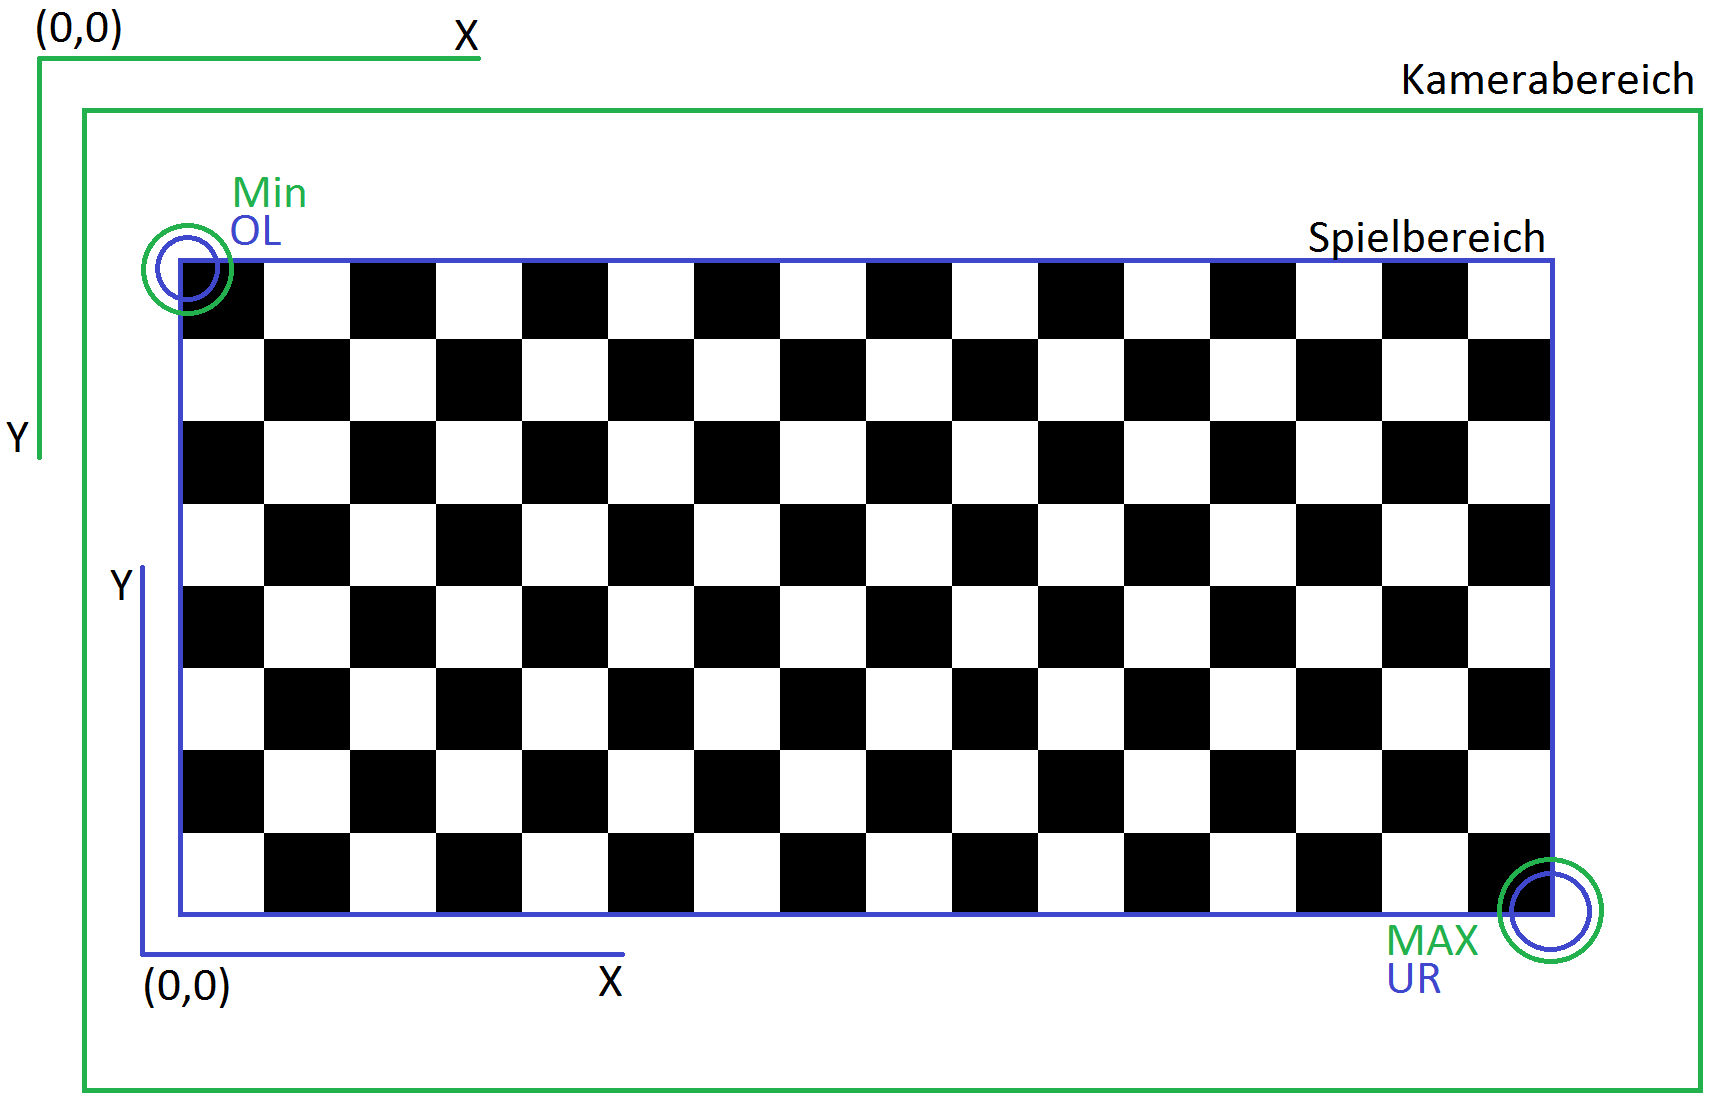
\includegraphics[scale=0.2]{bilder/schachbrettkamera.png}
		\caption{Kamera- und Spielkoordinatensystem}
	\end{figure}
\end{frame}
\begin{frame}{Erkennung des Queues}
\textbf{Problem:} Damit der Spieler die Kugeln mit dem Queue spielen kann, muss dieser im Kamerabild erkannt werden

\pause

\textbf{Unsere Lösung}:
\begin{itemize}
	\item[1.] Queue vom Hintergrund des Bildes segmentieren\\
	\pause
	$\implies$ zur Vereinfachung ist der Queue schwarz gefärbt
	\pause
	\item[2.] Hauptachse des Queues bestimmen
	\pause
	\item[3.] Durch die Hauptachse die beiden Endpunkte des Queues bestimmen
	\pause
	\item[4.] Die Endpunkte in Spielkoordinaten transformieren
	\pause
	\item[5.] Mit \textbf{beiden} Endpunkten die übliche Kollision ausführen
	
\end{itemize}
\end{frame}

\begin{frame}{Erkennung des Queues: Lösung}
\begin{itemize}
	\item [1.] Queue vom Hintergrund des Bildes segmentieren:
\end{itemize}
\begin{center}
\visible<1->{\stackunder[5pt]{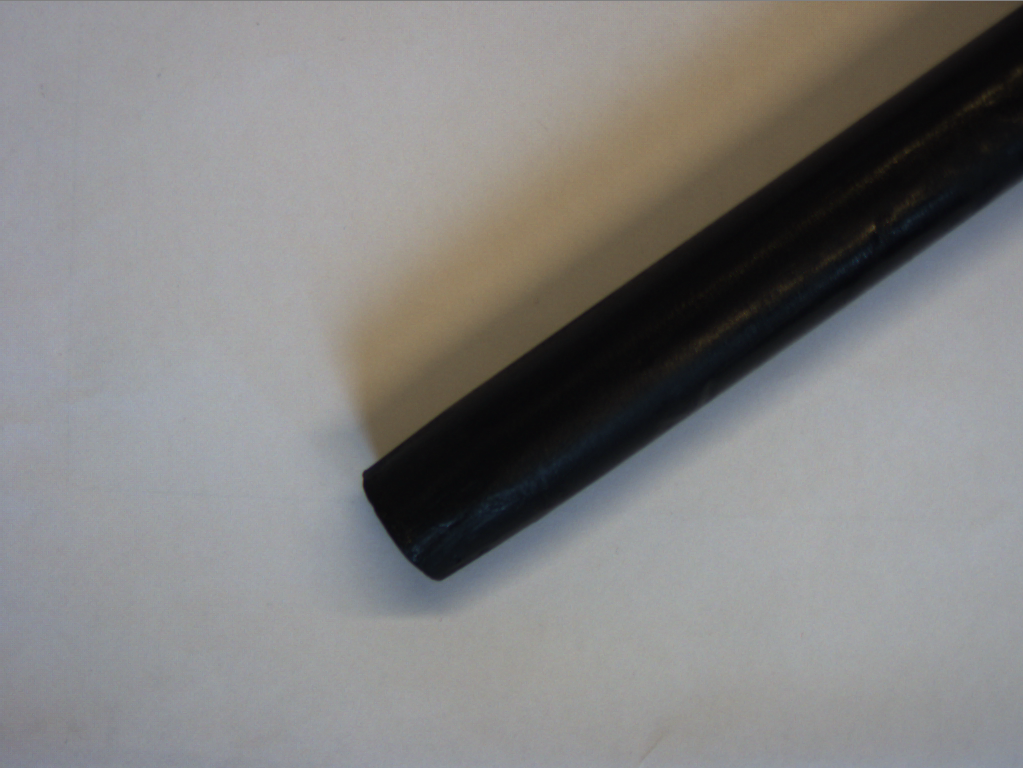
\includegraphics[height=2.3cm]{bilder/queue_orig.png}}{Kamerabild}}
\visible<2->{\stackunder[5pt]{
\includegraphics[height=2.3cm]{bilder/queue_thresholded.png}}{Segmentierung}}
\visible<3->{\stackunder[5pt]{
\includegraphics[height=2.3cm]{bilder/queue_close.png}}{Closing}}
\end{center}
\end{frame}
\begin{frame}{Kollision mit Queue: Lösung}
\begin{itemize}
	\item [2.] Hauptachse des Queues bestimmen\\
	$\implies$ durch Hauptkomponentenanalyse (PCA)
	
	\item [3.] Durch die Hauptachse die beiden Endpunkte des Queues bestimmen
\end{itemize}
\begin{center}
	\visible<1->{\stackunder[5pt]{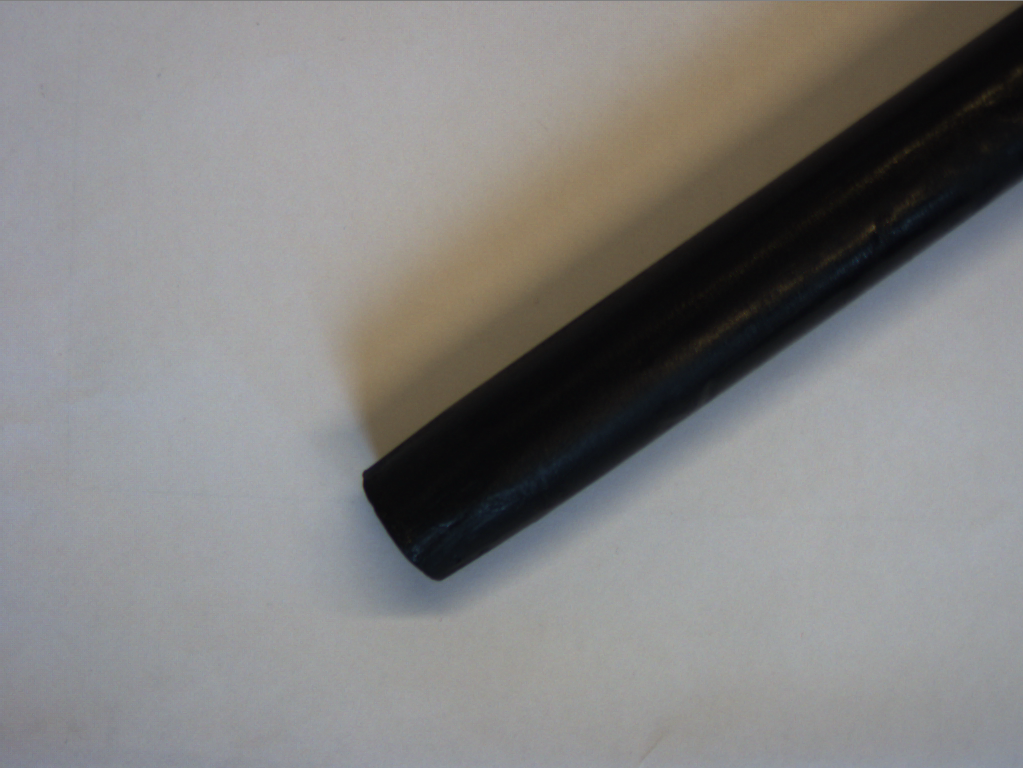
\includegraphics[height=2.3cm]{bilder/queue_orig.png}}{Kamerabild}}
	\visible<2->{\stackunder[5pt]{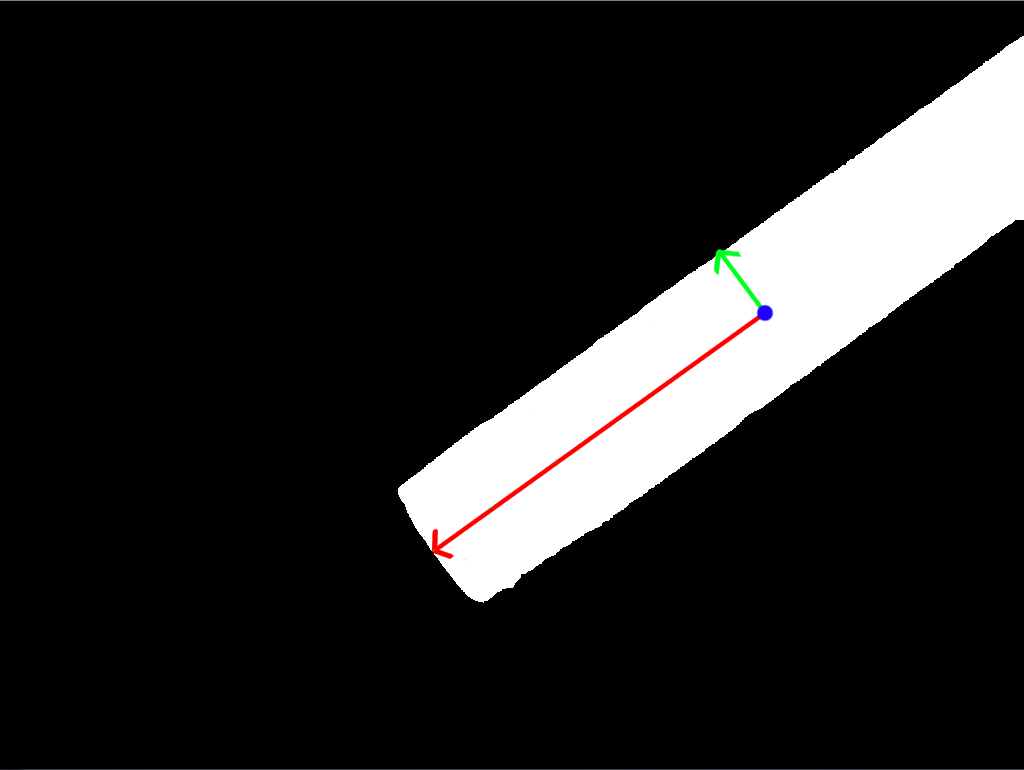
\includegraphics[height=2.3cm]{bilder/queue_pca_1.png}}{Ergebnis PCA}}
	\visible<3->{\stackunder[5pt]{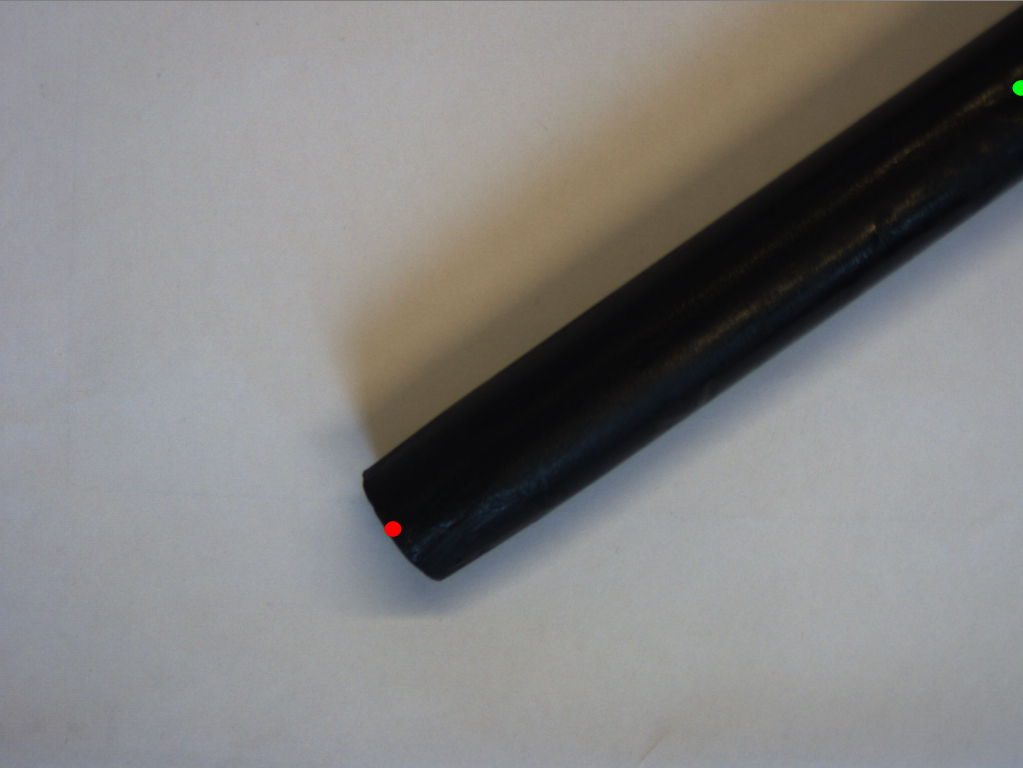
\includegraphics[height=2.3cm]{bilder/queue_pca_2.png}}{Bestimmte Endpunkte}}
\end{center}
\end{frame}

\begin{frame}{Erkennung des Queues: Lösung}
\begin{itemize}
	\item[4.] Die Endpunkte in Spielkoordinaten transformieren
	\item [5.] Mit den Endpunkten übliche Kollision ausführen	
\end{itemize}
\pause
\textbf{Problem:} Aufnahmen nur mit 24 Bildern pro Sekunde möglich\\
$\implies$ Kollisionen bei schneller Bewegung wird eventuell nicht erkannt!
\pause
\textbf{Lösung:}  Berechnung des Kollisionspunktes durch Interpolation
\begin{center}
	\visible<4->{\stackunder[5pt]{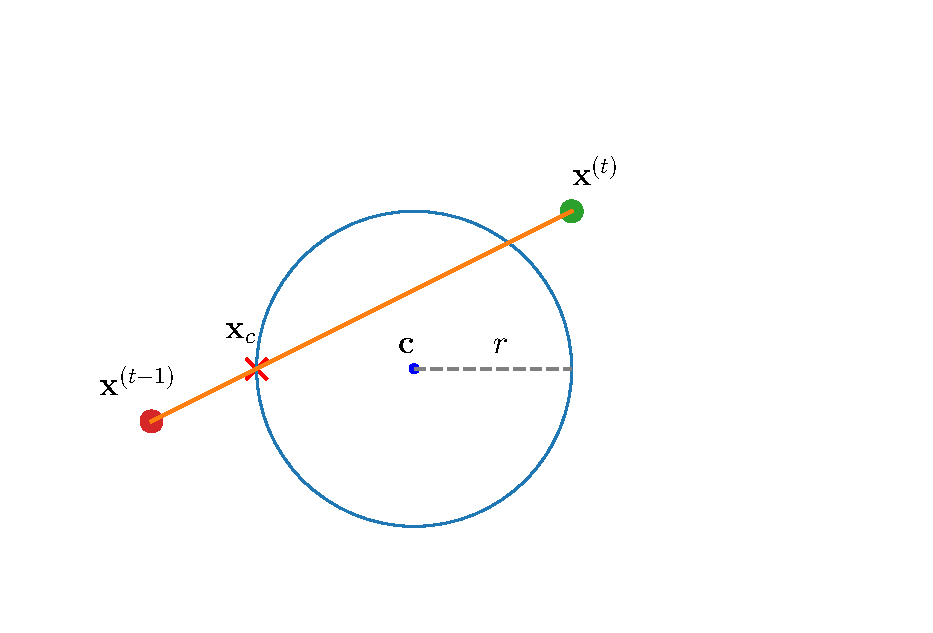
\includegraphics[height=2.7cm]{bilder/hit.eps}}{Kollision}}
	\visible<5->{\hspace{-0.7cm}\stackunder[5pt]{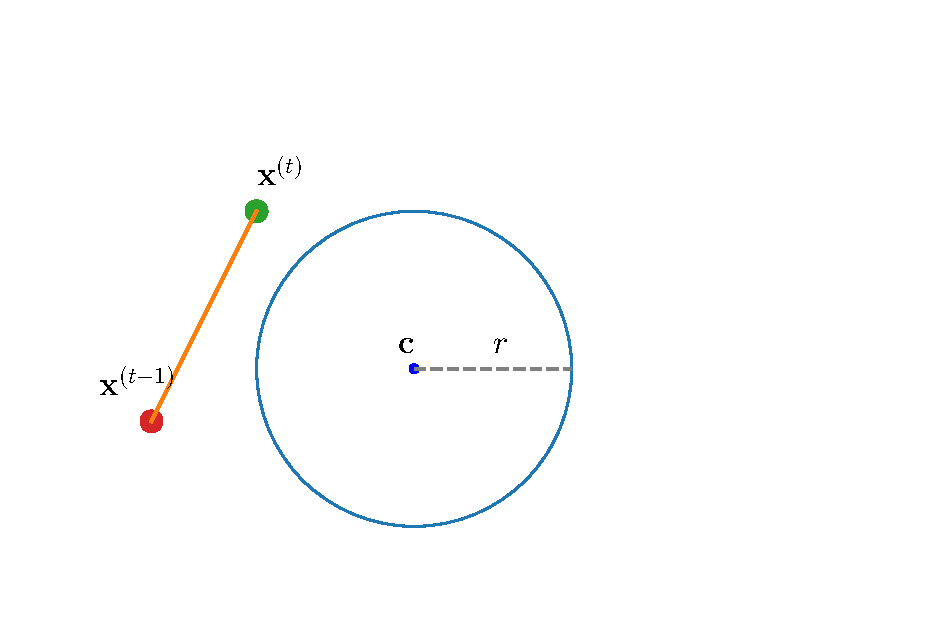
\includegraphics[height=2.7cm]{bilder/nohit.eps}}{Keine Kollision}}
	\visible<6->{\hspace{-1.2cm}\stackunder[5pt]{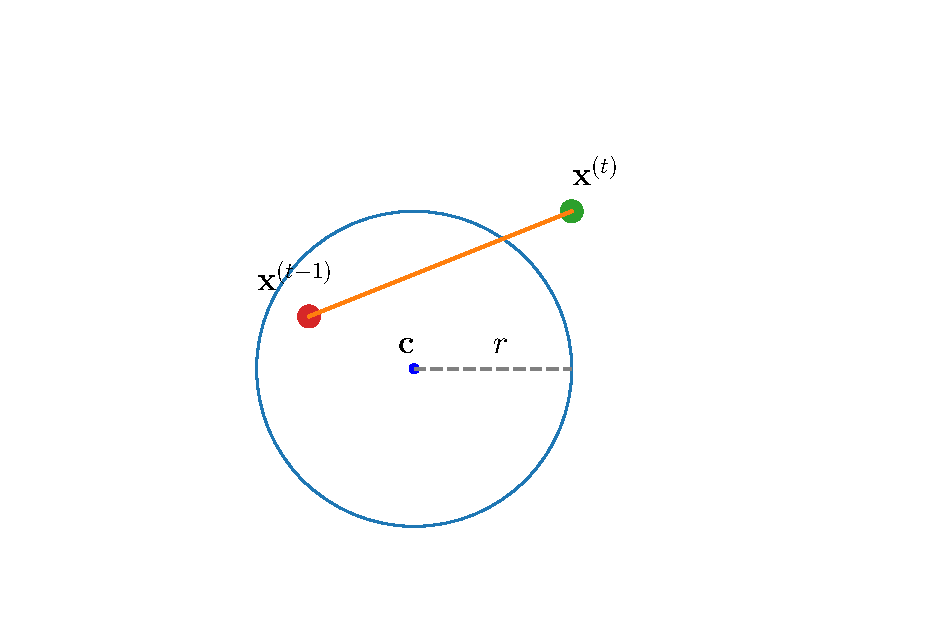
\includegraphics[height=2.7cm]{bilder/exitwound.eps}}{Keine Kollision}}
\end{center}
\end{frame}
\begin{frame}{Erkennung des Queues: Fazit}
	Die vorgestellte Lösung würde sich noch verbessern lassen:
	\begin{itemize}
		\pause
		\item Segmentierung  (und damit alle folgenden Schritte) stark von der Umgebung abhängig\\
		$\implies$ Verbesserung z.B. durch markerbasierte Erkennung
		\pause
		\item Wiederholfrequenz/Belichtungszeit der Kamera verursacht Bewegungsunschärfe\\
		$\implies$ Ungenauigkeit der Erkennung
	\end{itemize}
\end{frame}



\section{Spielregeln und Benutzerinteraktion}
Damit die Benutzerinteraktion funktioniert, müssen zunächst die Spielregeln ins Spiel eingebunden werden. Das Spiel das 8er- Ball-Billiard: \\
 8er Ball wird mit einem Spielball (weiss) und 15 nummerierten farbigen Kugeln gespielt. 14 der farbigen Kugeln werden in zwei Gruppen eingeteilt. Nr. 1 bis 7 sind vollfarbige (volle) Kugeln. Nr.9 bis 15 sind gestreiftfarbige (halbe) Kugeln. Zu Beginn werden alle 15 farbigen Bälle mit dem Dreieck so aufgestellt, dass die vorderste Kugel des Dreiecks auf dem Fusspunkt zu liegen kommt. Ziel des Spieles ist es, zuerst eine Serie von vollen oder halben Bällen und zuletzt den 8er Ball in die Löchern zu versenken. Jeweils der Gewinner eines Spieles eröffnet das nächste Spiel( Alternativ kann auch abwechslungsweise angespielt werden).

\subsection{Spielregeln}
Sobald der erste Spieler seinen Zug gemacht hat, started das Spiel.
Sollte der Spieler einen Ball eingelocht haben, überprüft die Spiellogik, ob es sich hierbei um eine vollen Ball handelt oder halben Ball. Entsprechend wird dabei der Balltyp des Spielers auf 'True' für einen vollen Ball oder auf 'False' für einen halben Ball gesetzt. Anschließend darf der derzeitig aktuelle Spieler einen weiteren Zug machen. \begin{equation}
BallTyp = \begin{cases}
True, & \text{ Für Volle Kugel } \\
False, & \text{ Für Halbe Kugel }
\end{cases}
\end{equation}

\begin{equation}
currentPlayer = \begin{cases}
0, & \text{ Für Ersten Spieler } \\
1, & \text{ Für Zweiten Spieler }
\end{cases}
\end{equation}

Hat der Spieler den Ball nicht eingelocht, dann wird der Spieler gewechselt.

dabei wird der BallType beim ersten spielzug nicht gesetzt, da niemand eine Farbe zugeordnet bekommen hat.
Um das Spiel zu Gewinnen muss man alle Kugeln eingelocht haben, die für den Spieler zugewiesen wurden. Die Letzte Kugel ist die Schwarze Kugel. Sollte diese versenkt worden sein, bevor alle Kugeln des Spielers versenkt sind, dann hat der Aktuelle Spieler entsprechen Verloren und ein Pop-up Fenster erscheint. Andernfalls hat Er  Gewonnen.

\subsection{Benutzerinteraktion}

Bevor ein Benutzer das Programm gestartet hat, müssen vorher einige voraussetzungen erfüllt werden. Das Programm benötigt zu ausführung eine Kamera. Diese wird zum Kalibrieren des Spielfeldes benötigt. Sollte die Kamera verbunden worden sein, so muss sie nun auf das Programm-Fenster zeigen. Zu Begin bei der Ausführung des Programms, wird ein Pop-up Fenster angezeigt, welche fragt ob die Kalibrierung gestartet werden kann(siehe Abbildung 3.6: Kalibrierung-Pop-up).
 \begin{figure}[h]
	\centering
	\caption{Kalibrierung-Pop-up}
	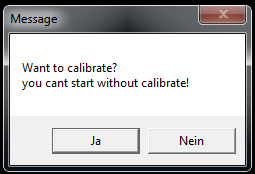
\includegraphics[width=\textwidth/3]{bilder/Calibrate-Popup.png}
\end{figure}\\
Mit dem Drücken des 'Ja'-Knopfes wird ein Signal richtung der Kamerakalibrierung geschickt und sie wird gestartet. Sollte 'Nein' gedrückt worden sein, so wird das Programm geschlosse, da das Programm die kalibrierung benötigt.
Nach der Kalibrierung wird ein weiteres Pop-up Fenster angezeigt, ob man das Spiel nun starten möchte. Wenn 'Ja' gedrückt wird, dann wird das ganze Spielfeld angezeigt. 
 \begin{figure}[h]
	\centering
	\caption{StartGame-Pop-up}
	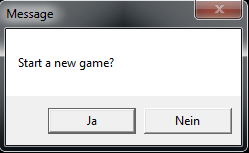
\includegraphics[width=\textwidth/3]{bilder/startGame-Popup.png}
\end{figure}\\
Nebenbei werden auch die Labels für den CurrentPlayer sowie des Balltypen angezeigt.
Das Spiel kann nun gespielt werden mit einem Queue. Hierbei muss man mit dem  Queue versuchen die weiße Kugel anzustoßen. Wichtig dabei ist, das die Kamera eingeschaltet bleiben muss.
\\\\\\
Als zusätliche funktion, hat der Spieler die möglichkeit mit der maus zu spielen(siehe Abb. 3.7: Maus Funktion), indem er sie entprechend zu der weißen kugel schlägt.
\begin{figure}[h]
	\centering
	\caption{Maus Funktion}
	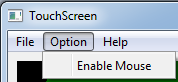
\includegraphics[width=\textwidth/3]{bilder/option-MenuBar.png}
\end{figure}\\\\
Unter File(siehe Abbildung 3.8: Start New Game) hat der Benutzer die möglichkeit das Spiel zurück zu setzten bzw. ein neues Spiel zu starten.
\begin{figure}[h]
	\centering
	\caption{Start New Game}
	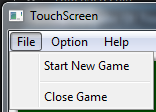
\includegraphics[width=\textwidth/3]{bilder/File-MenuBar.png}
\end{figure}\\





\begin{frame}[c]
\frametitle{Literatur}

\nocite{*}
\bibliographystyle{alphadin}
\bibliography{literatur}

\end{frame}

\end{document}
